\chapter{Discussion\label{discussion}}


\section{Type annotating Python programs} 

Research on Python Type annotations focuses on how they are used, and their benefits and adoption patterns. It is rare to analyse why they are adopted.


\section{Why choose Python, and then try to statically type it?}

Developers are not actually trying to completely statically type Python programs. As can be seen from the amount of type errors present in most Python projects in the wild\cite{rak-amnouykit_taleoftwo_2020, di_grazia_evolution_2022}, developers are utilizing the fact that a gradual type system enables gradually typing projects.

\subsection{Why use Python}
Python is popular for a multitude of reasons:

Its design goals have lead to a programming language that is easy to learn, quick to write, and simple to read. Effectively no popular statically typed languages have a similar design focus on developer experience.

The ease of learning Python leads to it being a popular teaching language, which enables it to provide a large developer base.

Useful packages are widely available. There is excellent support for various use cases, including scientific computing, machine learning, web development, desktop software development, and automation. \comment{TODO: tää ei nyt oo ihan hirveen vakuuttava}

\begin{figure}[h!]
    \centering
    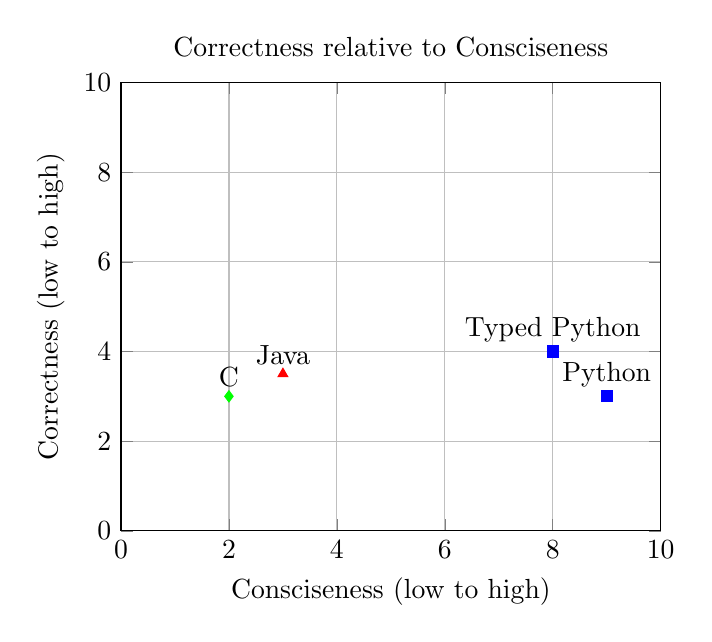
\begin{tikzpicture}
        \begin{axis}[
            xlabel={Consciseness (low to high)},
            ylabel={Correctness (low to high)},
            xmin=0, xmax=10,
            ymin=0, ymax=10,
            grid=major,
            legend pos=north west,
            title={Correctness relative to Consciseness}
        ]
        % Points for each language
        \addplot[only marks, mark=square*, color=blue] coordinates {(9, 3)}; % Python
        \addplot[only marks, mark=square*, color=blue] coordinates {(8, 4)}; % typed Python
        \addplot[only marks, mark=triangle*, color=red] coordinates {(3, 3.5)}; % Java
        \addplot[only marks, mark=diamond*, color=green] coordinates {(2, 3)}; % C
        % \addplot[only marks, mark=star, color=purple] coordinates {(1, 1)}; % asm
    
        % Adding labels for languages
        \node at (axis cs:9,3) [anchor=south] {Python};
        \node at (axis cs:8,4) [anchor=south] {Typed Python};
        \node at (axis cs:3,3.5) [anchor=south] {Java};
        \node at (axis cs:2,3) [anchor=south] {C};
        % \node at (axis cs:1,1) [anchor=south] {asm};
        \end{axis}
    \end{tikzpicture}
    \caption{A comparison of programming languages on consciseness and correctness.}
    \label{fig:language_comparison}
\end{figure}

\comment{Because of the fact that I don't have data to place the "Typed Python" on the figure properly, this feels a lot less informative and scientific than I originally thought. Maybe cut.}

Demonstrative figure \ref{fig:language_comparison} describes Python and Typed Python relative correctness and consciseness properties compared to other programming languages. Correctness refers to how many constructs and validations the language provides to ensure that programs are correct. Consciseness refers to the amount of required source code to achieve a certain function.

The figure is based on a study of various programming languages performance on Rosetta Code tasks \cite{nanz_comparative_2015}. They do not generalize to generic programs, but they are indicative and the relations are consistent with other research \cite{ray_codequality_2014}. (All the Python code in the study was untyped, since Python type annotations were not adopted before 2015. Typed Python was not researched in the study, and is a hypothetical addition.)

Python has apparently managed to arrive at a useful compromise on readability, expressivity and syntactic noise. Gradual typing provides a way to increase readability and correctness, with a cost of additional syntactic noise.

\subsection{Gradually typing Python}
Benefits of gradual typing: Gradual types work as documentation for internal and external APIs. Gradual types can be utilized to focus correctness efforts in the code base to the spots where they make most sense \cite{di_grazia_evolution_2022}.

\comment{TODO: expand on benefits / features of gradual typing}

\comment{\subsection{Why type check Python} TODO: type checking Python is easier than ever due to tooling improvements (Take some text from part 2.3.1 to here)}